\chapter{شبکه‌های عصبی عمیق}\label{chap:4}

\section{مقدمه}\label{sec:4-1}
شبکه‌های عصبی مصنوعی\LTRfootnote{Artificial Neural Networks (ANN)} یکی از مهم‌ترین زیرشاخه‌های یادگیری ماشین هستند که ساختار و عملکرد آن‌ها از شبکه‌های عصبی بیولوژیکی مغز انسان الهام گرفته شده است\cite{goodfellow2016deep} این شبکه‌ها از تعداد زیادی واحدهای پردازشی ساده به نام یاخته عصبی\LTRfootnote{Neuron}
 تشکیل شده‌اند که به صورت شبکه‌ای به هم متصل هستند. قدرت اصلی شبکه‌های عصبی مصنوعی در توانایی آن‌ها برای یادگیری الگوهای پیچیده و غیرخطی از درون داده‌ها نهفته است، که این ویژگی آن‌ها را برای حل مسائل پیچیده‌ای نظیر بینایی ماشین، پردازش زبان طبیعی و تشخیص گفتار به ابزاری بی‌بدیل تبدیل کرده است.

\section{یاخته عصبی مصنوعی}\label{sec:4-2}
واحد پایه‌ای و سازنده شبکه‌های عصبی مصنوعی، یاخته عصبی مصنوعی 
\LTRfootnote{Perceptron} 
نام دارد. برای درک بهتر نحوه عملکرد یاخته عصبی مصنوعی، می‌توان ساختار آن را با یک یاخته عصبی زیستی مقایسه کرد. 
همان‌طور که در \figurename~\ref{pic5} مشاهده می‌شود، می‌توان اجزای یک یاخته عصبی طبیعی (\figurename~\ref{subpic3}) را با معادل‌های ریاضی و منطقی آن در یک یاخته عصبی مصنوعی (\figurename~\ref{subpic4}) تطبیق داد. در شبکه عصبی زیستی، دارینه‌ها\LTRfootnote{Dendrites} وظیفه دریافت سیگنال‌ها از یاخته‌های عصبی دیگر را بر عهده دارند که این بخش در یاخته عصبی مصنوعی معادل موج‌های ورودی است. هسته\LTRfootnote{Nucleus} یا بدنه سلول، پردازش موج‌ها را انجام می‌دهد که در مدل مصنوعی با تابع جمع‌کننده خطی و تابع فعال‌ساز جایگزین شده است. در نهایت، آسه\LTRfootnote{Axon} که سیگنال خروجی را به سایر سلول‌ها منتقل می‌کند، معادل خروجی نهایی یاخته عصبی مصنوعی است.
\begin{figure}[H]
	\centering
	\begin{subfigure}{0.48\textwidth}
		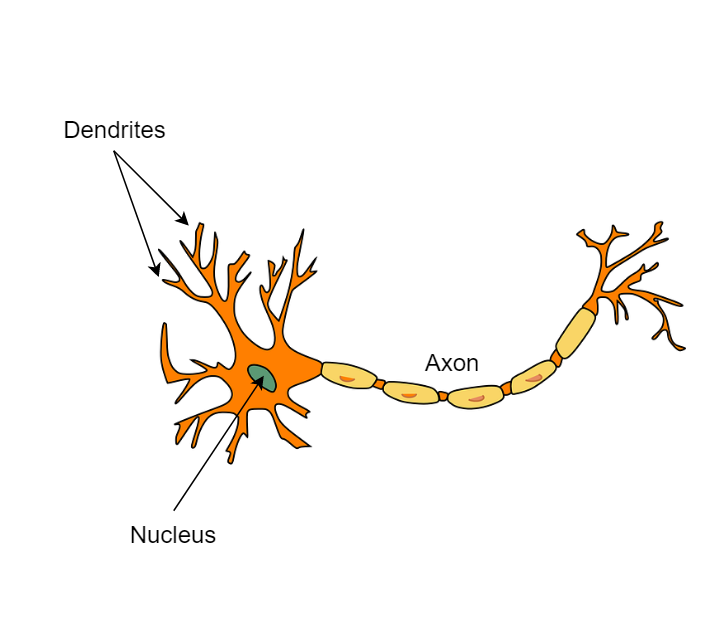
\includegraphics[width=\linewidth, height=7cm]{pic3}
		\caption{ساختار یک یاخته عصبی بیولوژیکی شامل دندریت‌ها، هسته و آکسون}
		\label{subpic3}
	\end{subfigure}
	\hfill
	\begin{subfigure}{0.48\textwidth}
		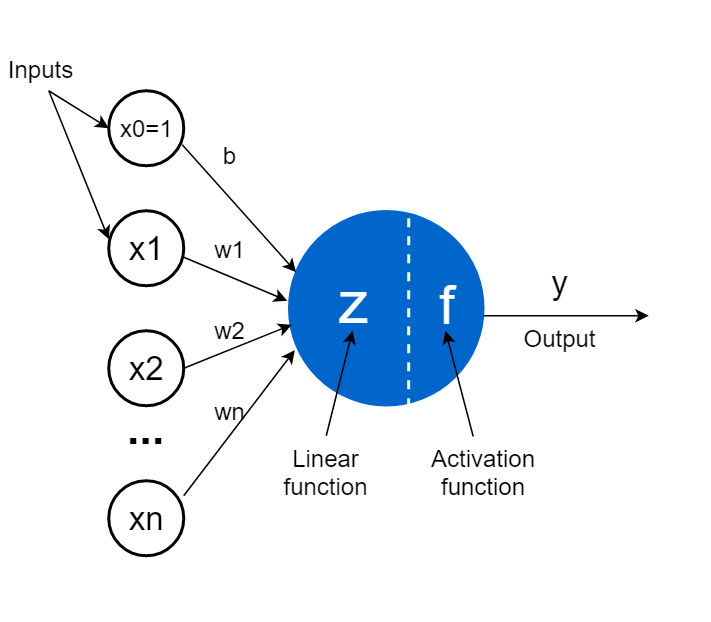
\includegraphics[width=\linewidth, height=7cm]{pic4}
		\caption{مدل ریاضی یک یاخته عصبی مصنوعی شامل ورودی‌ها، وزن‌ها، جمع‌کننده خطی و تابع فعال‌ساز}
		\label{subpic4}
	\end{subfigure}
	\caption{ساختار یاخته عصبی طبیعی در سیستم عصبی و مدل‌سازی یاخته عصبی مصنوعی}
	\label{pic5}
\end{figure}

از نظر ریاضی، عملکرد یک یاخته عصبی مصنوعی را می‌توان با استفاده از رابطه \eqref{eq18} بیان کرد:

\begin{equation} \label{eq18}
	y = f\left( \sum_{i=1}^{n} w_i x_i + b \right) = f(W^T X + b)
\end{equation}

در این معادله:
\begin{itemize}
	\item متغیر $X = [x_1, x_2, \dots, x_n]^T$ نشان‌دهنده بردار ورودی‌ها است.
	\item متغیر $W = [w_1, w_2, \dots, w_n]^T$ بردار وزن‌های متصل به هر ورودی را نشان می‌دهد که اهمیت هر موج ورودی را تعیین می‌کند.
	\item پارامتر $b$ (سوگیری\LTRfootnote{Bias})
	 مقداری است که به مجموع خطی اضافه می‌شود تا انعطاف‌پذیری مدل را برای برازش بهتر داده‌ها افزایش دهد.
	\item تابع $f$ همان تابع فعال‌ساز\LTRfootnote{Activation Function}
  ~است که ویژگی‌های غیرخطی را به خروجی مدل اضافه کرده و خروجی نهایی یعنی $y$ را تولید می‌کند.
\end{itemize}


\section{شبکه‌های عصبی چندلایه}\label{sec:4-3}
با وجود اینکه یک یاخته عصبی مصنوعی به تنهایی می‌تواند مسائل ساده و خطی را حل کند، اما برای یادگیری الگوهای پیچیده در داده‌های واقعی، به شبکه‌ای از این یاخته‌های عصبی نیاز داریم. اتصال چندین یاخته عصبی به یکدیگر در لایه‌های مختلف، ساختاری را به نام شبکه‌های عصبی چندلایه\LTRfootnote{Multilayer Perceptron (MLP)} شکل می‌دهد. 

\subsection{ساختار لایه‌ها}\label{subsec:4-3-1}
در یک شبکه عصبی معیار، یاخته‌های عصبی در سه نوع لایه مختلف دسته‌بندی می‌شوند که هر کدام وظیفه خاصی بر عهده دارند:

\begin{itemize}
	\item \textbf{لایه ورودی\LTRfootnote{Input Layer}:} این لایه نقطه آغازین شبکه است و وظیفه دریافت داده‌های خام را بر عهده دارد. تعداد یاخته‌های عصبیِ این لایه دقیقاً برابر با تعداد ویژگی‌های\LTRfootnote{Features} داده‌های ورودی ما است و هیچ‌گونه پردازشی روی داده‌ها انجام نمی‌دهد.
	
	\item \textbf{لایه‌های پنهان\LTRfootnote{Hidden Layers}:} این لایه‌ها بین ورودی و خروجی قرار دارند و قلب تپنده شبکه عصبی محسوب می‌شوند. وظیفه اصلی استخراج الگوها و ویژگی‌های پنهانِ داده‌ها بر عهده این بخش است. اگر یک شبکه عصبی بیش از یک لایه پنهان داشته باشد، به آن شبکه عصبی عمیق\LTRfootnote{Deep Neural Network (DNN)} گفته می‌شود و فرآیند آموزش آن را یادگیری عمیق\LTRfootnote{Deep Learning} می‌نامند.
	
	\item \textbf{لایه خروجی\LTRfootnote{Output Layer}:} نتایج نهاییِ پردازشِ شبکه، از این لایه به دست می‌آید. تعداد یاخته‌های عصبیِ لایه خروجی به نوع مسئله بستگی دارد؛ مثلاً در یک مسئله پیش‌بینی قیمت (رگرسیون\LTRfootnote{Regression}) تنها یک یاخته عصبی دارد، اما در مسئله تشخیص اعداد $0$ تا $9$ (دسته‌بندی)، شامل $10$ یاخته عصبی خواهد بود.
\end{itemize}

\subsection{توابع فعال‌ساز رایج}\label{subsec:4-3-2}
همان‌طور که در رابطه \eqref{eq18} دیدیم، توابع فعال‌ساز برای ایجاد خاصیت غیرخطی در شبکه استفاده می‌شوند. بدون وجود این توابع، هرچند شبکه ما لایه‌های بسیار زیادی داشته باشد، باز هم خروجیِ نهایی صرفاً یک ترکیب خطیِ ساده از ورودی‌ها خواهد بود و شبکه نمی‌تواند مسائل پیچیده دنیای واقعی را حل کند. در ادامه چهار مورد از پرکاربردترین توابع فعال‌ساز با بیانی ساده معرفی می‌شوند:

\textbf{۱. تابع سیگموئید \LTRfootnote{Sigmoid}} \\
این تابع، هر عدد ورودی را به یک مقدار خروجی در بازه $(0, 1)$ فشرده می‌کند. به دلیل همین ویژگی، معمولاً از این تابع برای مسائلی استفاده می‌شود که نیاز به پیش‌بینی احتمال وقوع یک اتفاق داریم. رابطه ریاضی آن به شکل زیر است:
\begin{equation} \label{eq19}
	f(x) = \frac{1}{1 + e^{-x}}
\end{equation}

\textbf{۲. تابع تانژانت هذلولوی\LTRfootnote{Hyperbolic Tangent (Tanh)}} \\
عملکرد این تابع بسیار شبیه به تابع سیگموئید است، با این تفاوت که خروجی‌های آن در بازه $(-1, 1)$ قرار می‌گیرند. این موضوع باعث می‌شود میانگین داده‌ها حول عدد $0$ متمرکز شود و معمولاً به یادگیری سریع‌تر شبکه کمک می‌کند:
\begin{equation} \label{eq20}
	f(x) = \frac{e^x - e^{-x}}{e^x + e^{-x}}
\end{equation}

\textbf{۳. تابع واحد خطی یکسوساز\LTRfootnote{Rectified Linear Unit (ReLU)}} \\
این تابع، امروزه محبوب‌ترین و پرکاربردترین تابع فعال‌ساز در شبکه‌های عمیق است. منطق این تابع بسیار ساده است: اگر ورودی مثبت باشد، خودِ آن عدد را برمی‌گرداند و اگر منفی باشد، خروجی را برابر صفر قرار می‌دهد. این سادگیِ ریاضی باعث افزایش چشمگیر سرعت محاسبات در رایانه\LTRfootnote{Computer} می‌شود:
\begin{equation} \label{eq21}
	f(x) = \max(0, x)
\end{equation}

\textbf{۴. تابع بیشینه هموار\LTRfootnote{Softmax}} \\
این تابع منحصراً در لایه خروجی برای مسائل دسته‌بندی چندطبقه‌ای\LTRfootnote{Multi-class Classification} استفاده می‌شود. این تابع خروجیِ تمام یاخته‌های عصبی لایه آخر را به گونه‌ای تنظیم می‌کند که مجموع آن‌ها دقیقاً برابر با عدد $1$ شود. به این ترتیب، می‌توانیم خروجی هر یاخته عصبی را به عنوان درصد احتمال تعلق داده به آن طبقه\LTRfootnote{Class} در نظر بگیریم:
\begin{equation} \label{eq22}
	f(x_i) = \frac{e^{x_i}}{\sum_{j=1}^{K} e^{x_j}}
\end{equation}
که در رابطه بالا، متغیر $K$ نشان‌دهنده تعداد کل طبقه‌ها است.

\subsection{توابع زیان}\label{subsec:4-3-3}
پس از آنکه ساختار شبکه عصبی و توابع فعال‌ساز مشخص شدند، نیازمند معیاری هستیم تا میزان خطای شبکه را در پیش‌بینی‌هایش ارزیابی کنیم. تابع زیان\LTRfootnote{Loss Function} وظیفه محاسبه این خطا را بر عهده دارد. 

همان‌طور که در فصل\ref{chap:3} به تفصیل مورد بررسی قرار گرفت و روابط ریاضی آن‌ها بیان شد، بسته به نوع مسئله از توابع متفاوتی استفاده می‌شود؛ در مسائل رگرسیون معمولاً از تابع خطای میانگین مربعات یعنی رابطه \eqref{eq15} و در مسائل دسته‌بندی از تابع زیان آنتروپی متقاطع یعنی رابطه \eqref{eq17} استفاده می‌شود. شبکه عصبی با استفاده از الگوریتم‌های بهینه‌سازی تلاش می‌کند تا مقدار این توابع را کمینه کرده و به بهترین پیش‌بینی دست یابد.
\section{آموزش شبکه عصبی}\label{sec:4-4}
اکنون که ساختار شبکه عصبی، توابع فعال‌ساز و معیار ارزیابی (تابع زیان) مشخص شدند، این پرسش مطرح می‌شود که شبکه چگونه مقادیر بهینه برای وزن‌ها ($W$) و سوگیری‌ها ($b$) را پیدا می‌کند تا خطای پیش‌بینی به حداقل برسد؟ فرآیند یادگیری در شبکه‌های عصبی عمیق طی یک چرخه تکرارشونده شامل دو مرحله اصلی انجام می‌شود: انتشار رو به جلو و پس‌انتشار خطا.

\subsection{انتشار رو به جلو و پس‌انتشار خطا}\label{subsec:4-4-1}
در مرحله \textbf{انتشار رو به جلو}\LTRfootnote{Forward Propagation}، داده‌های ورودی وارد شبکه شده و لایه به لایه در شبکه جلو می‌روند تا در نهایت یک خروجی (پیش‌بینی) تولید شود. سپس با استفاده از تابع زیان، میزان خطای این پیش‌بینی نسبت به مقدار واقعی محاسبه می‌گردد.

پس از محاسبه خطا، مرحله \textbf{پس‌انتشار خطا}\LTRfootnote{Backpropagation} آغاز می‌شود. این الگوریتم که ستون فقرات یادگیری عمیق محسوب می‌شود\cite{rumelhart1986learning}، با استفاده از قاعده زنجیره‌ای در حسابان\LTRfootnote{Chain Rule}، مشتق (گرادیان) تابع زیان را نسبت به تک‌تک وزن‌ها و سوگیری‌های موجود در شبکه از لایه آخر به سمت لایه اول محاسبه می‌کند. این گرادیان‌ها نشان می‌دهند که هر وزن چقدر در ایجاد خطای نهایی سهم داشته است و برای کاهش خطا باید در چه جهتی تغییر کند.

\subsection{الگوریتم‌های بهینه‌سازی}\label{subsec:4-4-2}
پس از محاسبه گرادیان‌ها در مرحله پس‌انتشار، شبکه برای به‌روزرسانی پارامترهای خود از الگوریتم‌های بهینه‌سازی\LTRfootnote{Optimization Algorithms} استفاده می‌کند. پایه و اساس اکثر این الگوریتم‌ها، روش \textbf{گرادیان کاهشی}\LTRfootnote{Gradient Descent} است. در این روش، پارامترهای شبکه در خلاف جهت شیب (گرادیان) تابع زیان حرکت می‌کنند تا به کمینه سراسری (کمترین میزان خطا) برسند. 

قانون پایه به‌روزرسانی وزن‌ها در الگوریتم گرادیان کاهشی به صورت رابطه \eqref{eq25} تعریف می‌شود:
\begin{equation} \label{eq25}
	w_{new} = w_{old} - \alpha \frac{\partial L}{\partial w}
\end{equation}
در این رابطه:
\begin{itemize}
	\item متغیر $w$ نشان‌دهنده وزنِ یاخته عصبی است.
	\item پارامتر $L$ همان تابع زیان است.
	\item عبارت $\frac{\partial L}{\partial w}$ نشان‌دهنده مشتق جزئی (گرادیان) تابع زیان نسبت به وزن است.
	\item متغیر $\alpha$ (آلفا) \textbf{نرخ یادگیری}\LTRfootnote{Learning Rate} نام دارد. این پارامترِ بسیار مهم، اندازه گام‌های شبکه را در مسیر کاهش خطا تعیین می‌کند. اگر $\alpha$ خیلی بزرگ باشد، ممکن است الگوریتم از نقطه بهینه عبور کند و اگر خیلی کوچک باشد، فرآیند یادگیری بسیار کند خواهد شد.
\end{itemize}

امروزه در شبکه‌های عصبی عمیق از نسخه‌های پیشرفته‌تر و تطبیق‌پذیرترِ گرادیان کاهشی استفاده می‌شود. یکی از محبوب‌ترینِ این روش‌ها، بهینه‌ساز \textbf{آدام}\LTRfootnote{Adam Optimizer} است.\cite{kingma2014adam}
 الگوریتم آدام با ترکیب مزایای روش‌های مختلف، نرخ یادگیری را برای هر پارامتر به صورت جداگانه و پویا در طول زمان تنظیم می‌کند که این امر منجر به همگرایی سریع‌تر و دقیق‌تر شبکه در مسائل پیچیده می‌شود.
\section{کاربردهای شبکه‌های عصبی عمیق}\label{sec:4-5}
با افزایش توان پردازشی رایانه‌ها و دسترسی به حجم عظیم داده‌ها (کلان‌داده‌ها)، شبکه‌های عصبی عمیق توانسته‌اند در بسیاری از حوزه‌های علمی و صنعتی تحولات چشمگیری ایجاد کنند. انعطاف‌پذیری این شبکه‌ها در یادگیری الگوهای پیچیده غیرخطی، باعث شده است تا در طیف وسیعی از مسائل به کار گرفته شوند. در ادامه به برخی از مهم‌ترین کاربردهای این شبکه‌ها اشاره می‌شود:

\begin{itemize}
	\item \textbf{امنیت شبکه و فضای سایبری\LTRfootnote{Cyber \& Network Security}:} یکی از کاربردهای بسیار مهم و رو به رشد یادگیری عمیق، تامین امنیت شبکه‌های کامپیوتری است. از این شبکه‌ها در سیستم‌های تشخیص نفوذ\LTRfootnote{Intrusion Detection Systems (IDS)} برای شناسایی رفتارهای غیرعادی و ترافیک مخرب استفاده می‌شود. شبکه‌های عصبی می‌توانند با تحلیل الگوهای ترافیک شبکه، حملاتی مانند منع سرویس توزیع‌شده\LTRfootnote{Distributed Denial of Service (DDoS)}، بدافزارها و فیشینگ را با دقت و سرعت بسیار بالایی نسبت به روش‌های سنتی شناسایی کنند.\cite{xin2018machine}
	\item \textbf{بینایی ماشین و پردازش تصویر\LTRfootnote{Computer Vision}:} از تشخیص چهره در تلفن‌های هوشمند گرفته تا سیستم‌های بینایی در خودروهای خودران و همچنین تشخیص تومورها در تصاویر پزشکی (مانند تصویربرداری تشدید مغناطیسی\LTRfootnote{MRI} و اشعه ایکس\LTRfootnote{X-Ray})، همگی از دستاوردهای شبکه‌های عصبی عمیق (به‌ویژه شبکه‌های پیچشی) هستند.
	
	\item \textbf{پردازش زبان طبیعی\LTRfootnote{Natural Language Processing (NLP)}:} درک و تولید زبان انسان توسط ماشین، ترجمه ماشینی (مانند مترجم گوگل)، دستیارهای صوتی هوشمند و چت‌بات‌های پیشرفته، همگی بر پایه معماری‌های عمیق شبکه‌های عصبی بنا شده‌اند.
\end{itemize}
